\documentclass{article}
\usepackage[a4paper, total={6.5in, 10in}]{geometry}
\usepackage{float}
\usepackage{amsmath}
\usepackage{enumitem}
\usepackage{graphicx}
\usepackage{placeins} % put this in your pre-amble
\usepackage{flafter}  % put this in your pre-amble
\usepackage{spverbatim}

\title{CS-E4410 Semantic Web-HW2}
\author{
  Erdogar, Can\      \texttt{625391}
}
\date{ 2 March 2017}
\usepackage{pgfplots}
\usepackage{tikz}
\usetikzlibrary{arrows,automata}

\begin{document}

\maketitle

\section{SPARQL basics}

\subsection{YASGUI application}

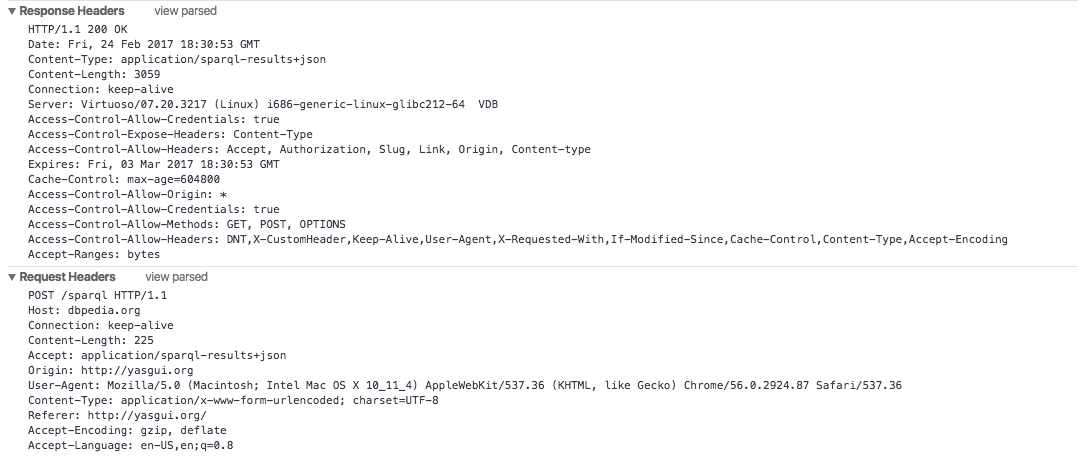
\includegraphics[width=\textwidth]{rdf-grapher.png}

The parameter name that is used for sending the SPARQL query in HTTP is POST request.

$ $

$ $

$ $

$ $

$ $

$ $


\subsection{SPARQL ASK}

\begin{verbatim}
PREFIX rdf: <http://www.w3.org/1999/02/22-rdf-syntax-ns#>
PREFIX rdfs: <http://www.w3.org/2000/01/rdf-schema#>
ASK
WHERE{
 ?g <http://www.w3.org/2000/01/rdf-schema#label> "The bombardment of Sveaborg"@en.
}
\end{verbatim}

There is such a resource which exists.

$ $

$ $

$ $

$ $

$ $

$ $

$ $

$ $

$ $

$ $
\subsection{SPARQL DESCRIBE}

\begin{verbatim}
PREFIX rdf: <http://www.w3.org/1999/02/22-rdf-syntax-ns#>
PREFIX rdfs: <http://www.w3.org/2000/01/rdf-schema#>
DESCRIBE
WHERE{
 ?g <http://www.w3.org/2000/01/rdf-schema#label> "The bombardment of Sveaborg"@en.
}
\end{verbatim}

Description is as follows,

\begin{spverbatim}
<http://ldf.fi/history/histo/p5084>
        a       <http://www.cidoc-crm.org/cidoc-crm/E5_Event> ;
        <http://www.w3.org/2000/01/rdf-schema#label>
                "Viaporin pommitus"@fi , "Sveaborg bombas"@sv , "The bombardment of Sveaborg"@en ;
        <http://purl.org/dc/elements/1.1/created>
                "2012-11-13T08:43:27.379+00:00"^^<http://www.w3.org/2001/XMLSchema#dateTime> ;
        <http://purl.org/dc/elements/1.1/description>
                "Krimin sotaan osallistunut brittiläis-ranskalainen laivasto purjehti Helsingin edustalle elokuussa 1855. Viaporin pommitus alkoi 9. elokuuta. Helsinkiläiset seuraisivat tapahtumia Ullanlinnan ja Kaivopuiston kallioilta. Aamupäivällä ruudin ja linnoituksessa syttyneiden tulipalojen savu peitti linnoituksen. Iltapäivällä Kustaanmiekalla rähähti ammusvarstoja. Pommitukset jatkuivat läpi yön ja palavat raketit valaisivat tulimerenä taivaan. Pommitukset päättyivät aamulla 11. elokuuta. Helsinkiläisten yllätykseksi liittoutuneiden laivasto ei yrittänyt maihinnousua, vaan purjehti pois. Helsingin kaupunki säilyi pommituksilta turvassa, mutta Viaporissa 55 ihmistä kuoli ja 204 haavoittui, minkä lisäksi rakennuksia tuhoutui. Viaporin komendantin alaisuudessa oli 15000 hengen miehistö, jonka käytössä oli 700 tykkiä. Vanhentuneen aseet eivät kantaneet vihollisen laivoihin asti. Krimin sodan myötä Viaporin merkitys laivastotukikohtana väheni." ;
        <http://purl.org/dc/elements/1.1/modified>
                "2012-11-14T08:16:22.995+00:00"^^<http://www.w3.org/2001/XMLSchema#dateTime> ;
        <http://www.cidoc-crm.org/cidoc-crm/P11_had_participant>
                <http://ldf.fi/history/histo/p5069> , <http://ldf.fi/history/histo/p5020> , <http://ldf.fi/history/histo/p5071> ;
        <http://www.cidoc-crm.org/cidoc-crm/P4_has_time-span>
                <http://ldf.fi/history/histo/p5061> ;
        <http://www.cidoc-crm.org/cidoc-crm/P7_took_place_at>
                <http://ldf.fi/history/kb/p157553> .
\end{spverbatim}
$ $

$ $
The CIDOC Conceptual Reference Model (CRM) provides definitions and a formal structure for describing the implicit and explicit concepts and relationships used in cultural heritage documentation. \\
E5 Event is used to indicate the changes of states in cultural, social or physical systems, regardless of scale, brought about by a series or group of coherent physical, cultural, technological or legal phenomena.\\


\subsection{Simple SPARQL SELECT}
\begin{verbatim}
PREFIX rdf: <http://www.w3.org/1999/02/22-rdf-syntax-ns#>
PREFIX rdfs: <http://www.w3.org/2000/01/rdf-schema#>
SELECT ?s
WHERE {
  ?s <http://www.w3.org/2000/01/rdf-schema#label> "2001: A Space Odyssey"@en .
  ?s rdf:type <http://www.wikidata.org/entity/Q11424>.
}

URI: http://www.wikidata.org/entity/Q103474
\end{verbatim}



\subsection{Simple SPARQL SELECT}

\begin{verbatim}
PREFIX rdf: <http://www.w3.org/1999/02/22-rdf-syntax-ns#>
PREFIX rdfs: <http://www.w3.org/2000/01/rdf-schema#>
SELECT ?s ?label
WHERE {
  ?s <http://www.w3.org/2000/01/rdf-schema#label> "2001: A Space Odyssey"@en .
  ?s rdf:type <http://www.wikidata.org/entity/Q11424>.
  ?s <http://www.wikidata.org/entity/P161c> ?g.
  ?g rdfs:label ?label.
  FILTER (lang(?label) = "en" )
}
\end{verbatim}

\subsection{Aggregates}
\begin{verbatim}
PREFIX rdf: <http://www.w3.org/1999/02/22-rdf-syntax-ns#>
PREFIX rdfs: <http://www.w3.org/2000/01/rdf-schema#>


SELECT ?g COUNT(?m) WHERE {
  ?s <http://www.w3.org/2000/01/rdf-schema#label> "2001: A Space Odyssey"@en .
  ?s rdf:type <http://www.wikidata.org/entity/Q11424>.
  ?s <http://www.wikidata.org/entity/P161c> ?g.
  ?g rdfs:label ?label.
  FILTER (lang(?label) = "en" )
  ?m <http://www.wikidata.org/entity/P161c> ?g.

}GROUP BY(?g)
\end{verbatim}

\section{Data transformation with SPARQL CONSTRUCT}

\section{Federated query}

\begin{verbatim}
PREFIX rdf: <http://www.w3.org/1999/02/22-rdf-syntax-ns#>
PREFIX rdfs: <http://www.w3.org/2000/01/rdf-schema#>
PREFIX itemcard: <http://www.cs.helsinki.fi/group/seco/ns/2004/03/18-esinekortti#>
PREFIX skos: <http://www.w3.org/2004/02/skos/core#>

SELECT ?cityname ?lat ?long (GROUP_CONCAT(?binded; SEPARATOR=" $ ") as ?itemlist)
WHERE{
  SERVICE <http://dbpedia.org/sparql>
  {
	?s <http://www.wikidata.org/entity/P625c> ?c.
    ?s <http://www.wikidata.org/entity/P373c> ?cityname.
    VALUES ?cityname {"Vantaa" "Kuopio"}
    ?c <http://www.wikidata.org/ontology#latitude> ?lat.
  	?c <http://www.wikidata.org/ontology#longitude> ?long
  }
  ?items rdf:type itemcard:Esinekortti.
  ?items itemcard:valmistuspaikka ?g.
  ?g skos:prefLabel ?cityname.
  ?items rdfs:label ?label. 
  ?items itemcard:www_kuvatiedosto_pieni_url ?url.
  BIND(CONCAT(?label, '#', ?url) AS ?binded).
  
}group by ?cityname ?lat ?long
\end{verbatim}

\section{Using a SPARQL endpoint with JavaScript}

I set the query value in initialize function to above query and set the endpoint to \textbf{http://ldf.fi/mufi/sparql} and it worked.

\section{Visualizing SPARQL results with YASGUI}

\begin{verbatim}
PREFIX dct: <http://purl.org/dc/terms/>
PREFIX dbc: <http://dbpedia.org/resource/Category:>
PREFIX dbo: <http://dbpedia.org/ontology/>
PREFIX : <http://dbpedia.org/resource/>

SELECT ?s COUNT(?g) AS ?number
WHERE{
 ?s dct:subject dbc:Cities_and_towns_in_Finland.
  ?g dbo:birthPlace ?s.
}GROUP BY ?s
ORDER BY DESC (?number)
LIMIT 20
\end{verbatim}

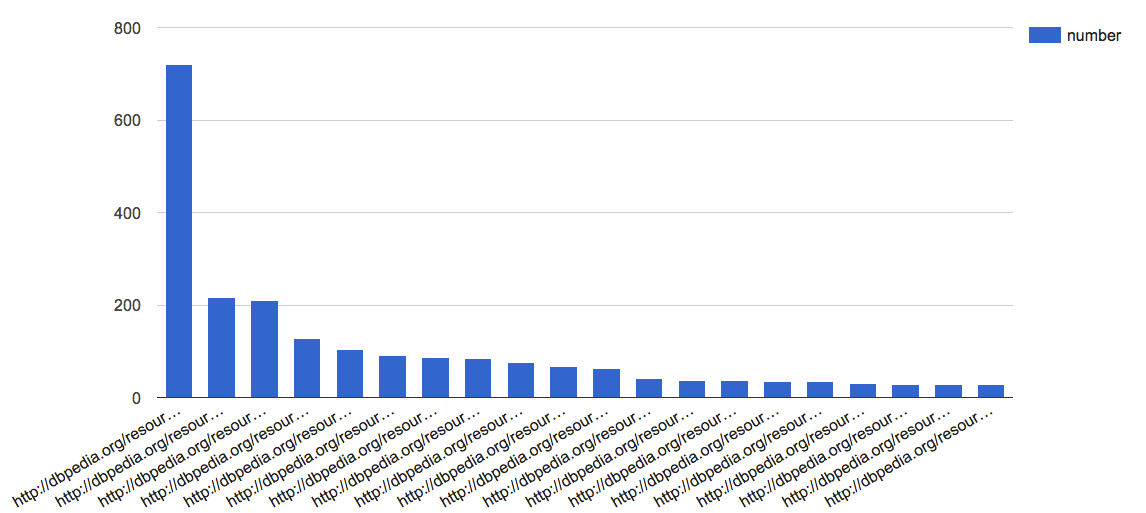
\includegraphics[width=\textwidth]{22.png}

\section{SPARQL Update}

\section{Serving RDF data}

\begin{verbatim}
SELECT ?g
WHERE{
?g <http://www.w3.org/2000/01/rdf-schema#label> "chaffinch"@en.
}
\end{verbatim}

returns \\

\begin{verbatim}
-------------------------------------------------------
| g                                                   |
=======================================================
| <http://www.yso.fi/onto/bio/FMNH_vernacular_367729> |
| <http://www.yso.fi/onto/bio/FMNH_381610>            |
-------------------------------------------------------
\end{verbatim}

\end{document}

​



